\DefineVerbatimEnvironment%
{Code}{Verbatim}{fontsize=\small,samepage=true,xleftmargin=1in}
\DefineVerbatimEnvironment%
{WrapCode}{Verbatim}{fontsize=\small,samepage=true,xleftmargin=0in}
\section{Introduction}

PBIO (Portable Binary Input/Output)/JIX (Just In time XML) is a system for
efficiently marshalling data for communication in a heterogeneous computing
environment.  This manual servers as both an introduction to using PBIO/JIX
and as a reference manual for the API.

\section{PBIO Basics}

The basic approach of the Portable Binary I/O library is relatively simple.
PBIO is record-oriented.  Writers (or encoders) of data must provide a
description of the names, types, sizes and positions of the fields in the
records they are writing.  On the writer's side this is done by ``registering
a format.''  Readers (or decoders) must provide similar information for the
records that they are interested in reading.  On the reading side, this is
done for each incoming format and is called ``setting a conversion,'' that
is, establishing a correspondence between the fields in the incoming records
and the fields in the local data structure into which the information is to
be placed.  No translation is done on the writer's end.  On the reader's
end, the format of the incoming record is compared with the format that the
program expects.  If there are discrepancies the PBIO read routine performs
the appropriate translations (conversions).
\paragraph{How does XML fit into the picture?}  PBIO record decoding semantics
are much like what you would get from using XML for data communication.  PBIO
transparently ignores extra fields that the decoder isn't expecting and
removes any dependence upon field ordering.  PBIO-encoded records can also be
queried to determine what fields and types they contain.  These features are
some of the most important advantages that drive the adoption of XML in
communication.  

However, XML uses an inefficient character-based data encoding to provide
these semantics.   The PBIO/JIX approach is quite different.  Instead of every
record containing the complete data and structure definition, as in an XML
document.  We separate the structure (XML markup) from the data.   The markup
is associated with the PBIO format and is only used if the record is to be
converted into XML.  This leverages the fact that most XML-producing
applications operate on their data in binary forms and only create XML just
before the data is to be transmitted.  In the PBIO approach, we register the
XML markup with the format.  The application then encodes the data with PBIO
instead of turning it into XML.  This process will be detailed in
Section~\ref{XML}. 

Because of the PBIO/JIX focus on high-performance applications, this document
is written using examples in C to transmit C structs.  In C++, the examples
work equally well using classes without methods instead of structs.

\subsection{High-level Constructs}
PBIO/JIX supports both file-oriented and online (network-based) data
interchange.  File-oriented PBIO is the most straightforward.  In this case
the highest-level PBIO construct is the \routine{IOFile}.  PBIO files are always
either read-only or write-only.  In writing a PBIO file, the application must
first register a format for records to be written and then may write records. 
In reading a PBIO file, an application must specify a conversion for records
in the file before they are read.  The \routine{IOFile} also controls the scope of
name resolution.  That is, the name ``Item'' may be associated with a
particular structure in one \routine{IOFile} and with a different structure in another
\routine{IOFile} without any conflict.

In some situations, such as when using PBIO as a data encoding mechanism for
network communication, a file-oriented abstraction is unworkable.  To handle
these situations, PBIO provides an abstraction called an \routine{IOContext}.
\routine{IOContext}s are very similar to \routine{IOFile}s except for two key differences:
\begin{itemize}
\item Instead of \routine{IOFile} read/write operations that take/put data directly
to/from a filesystem, \routine{IOContext}s have encode/decode operations.  In
encode/decode, PBIO plays no role in actual data storage or transmission.
Instead, the application is responsible for actually moving the encoded data
from place to place.
\item While \routine{IOFile}s are either read-only or write-only, a single \routine{IOContext}
can be used for both encoding and decoding.
\end{itemize}

Internally to PBIO, \routine{IOFile} and \routine{IOContext} are the same data structure.
Because PBIO operations like registering formats and setting conversions are
common to both, the PBIO API generally provides similar routines for
\routine{IOFile}s and \routine{IOContext}s.  In {\it some} more unusual situations only one
routine is provided and an application can safely cast between the two data
types.

Because the \routine{IOFile} interface is somewhat conceptually easier and files are
a handy storage mechanism, the remainder of this section will describe the
basics of PBIO in the context of \routine{IOFile}s.  The \routine{IOContext} functionality
will next appear in Section~\ref{iocontext}.

\subsection{Supported Data Types\label{sec:datatypes}}

The PBIO routines support record formats consisting of fields of the following
basic data types: ``integer'', ``unsigned integer'', ``float'', ``char'',
``enumeration'' and ``string''.  Note that {\em field type} here is separate
from {\em field size} so that both the native C types ``int'' and ``long'' are
``integer'' types.  ``char'' is essentially treated as a small ``integer''
except that the {\bf IOdump} program and other data-to-text subroutines will
print it as a character. 
``enumeration'' is also treated as an integer and there is currently no
mechanism to apprise the IO routines of the symbolic names associated with the
values.  ``string'' is a C-style zero-terminated variant-length string.  Both
NULL and zero-length strings are handled appropriately.  

There is no prohibition on the use of types not listed here.  However
translation and display are not available for other than the built-in types.

\subsection{Field Lists\label{sec:fieldlist}}
A record format is characterized by a field list.  Each field is specified by
its name, basic data type, the field's size and offset in the record.  The
field name and basic data type are specified with strings.  The size and
offset are integers.  Below is an example structure for a record and the
corresponding field list:
\begin{verbatim}
typedef struct _first_rec {
    int         i;
    long        j;
    double      d;
    char        c;
} first_rec, *first_rec_ptr;

static IOField field_list[] = {
    {"i", "integer", sizeof(int), IOOffset(first_rec_ptr, i)},
    {"j", "integer", sizeof(long), IOOffset(first_rec_ptr, j)},
    {"d", "float",   sizeof(double), IOOffset(first_rec_ptr, d)},
    {"c", "integer", sizeof(char), IOOffset(first_rec_ptr, c)},
    {NULL, NULL, 0, 0},
};
\end{verbatim}
\index{IOField}\index{IOOffset}

The ``IOOffset'' macro simply calculates the offset of a field in a structure
using compile-time information.  Its use is recommended to avoid
hand-calculating and hard-coding offsets.  The order of fields in the field
list is not important.  It is not even necessary to specify every field
in a structure with an entry in the field list. Unspecified fields at the end
of the structure may not be written to the IO file.  Unspecified fields
at the beginning or in the middle of a structure will be written to the IO
file, but no information about them will be available.\footnote{{\it Nota
Bene:} This behavior results because PBIO treats base data records (not
strings or other dynamically sized elements) as a contiguous memory block
for efficiency.  The compiler may leave ``holes'' in the data block to
preserve the required alignment for some data types.  Because PBIO puts the
data on the wire as a contiguous block, the values in these ``holes'' are put
on the wire as well.  Fields in the record that are not described to PBIO
via the field list are simply treated as larger ``holes''.  Note that
relying on the behavior of PBIO with respect to values in these ``holes''
is erroneous and can have unpredictable results.  For example, ``hole
values'' may appear to be transmitted along with the data in an exchange
between homogeneous systems, yet not in other cases.}
\subsection{Formats and Conversions}

While field lists characterize the layout of records, it would be inefficient
to process the string-oriented field list on every record read or write.  To
avoid this inefficiency, field lists must be analyzed prior to reading or
writing data.  For writing/encoding, field lists are ``registered'' with a
particular output file with the call \routine{register\_IOrecord\_format()}.  This
call specifies a name to be associated with the record format in the file and
returns a handle, of the type \routine{IOFormat}.  The returned \routine{IOFormat} is used in
the 
\routine{write\_IOfile()} call and specifies the format of the data to be written to the
file.  The names of record formats must be unique within a PBIO file and are
used on the reading end to identify specific record format within the file.
Because there is no translation upon write in the PBIO scheme, the field list
which governs the writing \routine{IOFormat} becomes the {\it file record format} in
the written file.

In the case of reading a PBIO file, IOConversions facilitate the common case
where the reading program knows, for the records in which it interested, the
names of both the record format and the fields within those format which it
requires.  For reading, the subroutine \routine{set\_IOconversion()} serves a
similar function as \routine{register\_IOrecord\_format()}.  However, instead of
the field list specifying the format of the records in the file, it specifies
the fields required {\it from} the file and the program format into which they
are to be converted.  The format name specified in the
\routine{set\_IOconversion()} call must match the name of a format in the file.
The record format in the file must contain {\it at least} all the fields
specified in the conversion field list.  If there are more fields in the file
record format than the reader specifies in the conversion, those additional
fields in file records are ignored.  For the fields that are common between
the formats, the PBIO library will perform any data rearrangement or conversion
that is required to convert the incoming binary file record into a native
record.  Reading programs {\it must} set a conversion for incoming data they
wish to have converted into comprehensible form.  

\subsection{Simple Read and Write Programs\label{sec:simple}}
Given the structure and field declarations above, a simple writer and reader
programs are shown in Figures~\ref{writer} and \ref{reader}.
\begin{figure}[bt]
\begin{Code}
int main(int argc, char **argv)
{
    IOFile iofile = open_IOfile("test_output", "w");
    IOFormat first_rec_ioformat;
    first_rec rec1;
    int i;

    first_rec_ioformat = register_IOrecord_format("first format", field_list, iofile);
    for(i=0; i<10; i++) {
        rec1.i = i;  rec1.j = 2*i; rec1.d = 2.727 + i; rec1.c = 'A' + 2*i;
        if(!write_IOfile(iofile, first_rec_ioformat, &rec1)) {
           printf("write failed\n");
        }
    }
    close_IOfile(iofile);
}
\end{Code}
\vspace*{-.25in}
\caption{A simple writer program.\label{writer}}
\index{open\_IOfile()}\index{register\_IOrecord\_format()}\index{write\_IOfile()}\index{close\_IOfile()}

\end{figure}
\begin{figure}[tbh]
\begin{Code}
void main(int argc, char **argv)
{
    IOFile iofile = open_IOfile("test_output", "r");
    first_rec rec1;
    int i;

    set_IOconversion(iofile, "first format", field_list, sizeof(first_rec));
    for(i=0; i<10; i++) {
        read_IOfile(iofile, &rec1);
        printf("rec had %d, %d, %g, %c\n", rec1.i, rec1.j, rec1.d, rec1.c);
    }
    close_IOfile(iofile);
}
\end{Code}
\vspace*{-.25in}
\caption{A simple reader program.\label{reader}}
\index{open\_IOfile()}\index{set\_IOconversion()}\index{read\_IOfile()}\index{close\_IOfile()}
\end{figure}
These simple programs handle the most common data transfer
situation.\footnote{Both the sample reader and writer programs use the routine
\routine{open\_IOfile()}, which is used for file-based data exchanges.  The routine
\routine{open\_IOfd()} takes an integer file descriptor instead of a filename as an
argument and is used for socket- or stream-based exchanges.}  
The source program supplies the complete specification of the data being
written.  The destination program specifies the fields that it is interested
in and their locations and sizes in the data structure in which it would like
them placed. Fields are matched by name.  If there are differences in
structure specifications, the PBIO routines perform the appropriate
conversions at the time of the read operation.  The reader program will read
the binary files produced by the writer program, despite potential difference
in: 
\begin{list}{$\bullet$\hfill}{\let\makelabel\descriptionlabel\setlength{\itemsep}{0in}\setlength{\topsep}{0in}}
\item byte ordering on the reading and writing architectures.
\item differences in sizes of datatypes (e.g. long and int).
\item compiler structure layout differences.
\end{list}
In the general case, the reading and writing program need not be using the
same structures at all, although all the fields that the reading program
specifies {\em must} actually exist in the data.  The IO routines can also
convert a float field to an integer and vice versa.  There is, of
course, the possibility of data loss in any conversion.  If the user requests
that an 8-byte integer in the data stream be placed in a 2-byte integer in the
program, the top 6 bytes will be lost.  A floating point value may not be
precisely representable as an integer nor a large integer by a floating point
value.  At present, loss of data occurs quietly, but future extensions may
address this issue.  Note that the reading program must set a conversion
for all record formats for which it wishes to use \routine{read\_IOfile()}.  If no
conversion is set, the \routine{read\_IOfile()} call will fail and the record will be
discarded.  

\section{More Complex Issues}
The programs in the presented previous section are sufficient to handle the
transmission of simple atomic data types in the simplest of circumstances.
This section will expand on that implementation basis with additional
facilities. 

\subsection{Strings and Memory Handling\label{stringmem}}

The sample programs presented above exercise all the basic data types
including ``string'', but it leaves open some questions about memory
management.  The principal complication in handling variable-length strings
is that exact storage requirements aren't known beforehand.  This isn't an
issue on the writing end, but on the reading end either the user must
provide memory for strings or it must be allocated by the PBIO library.  It
is possible to use either approach with PBIO.  In particular, if records
containing string datatypes are read using the \routine{read\_IOfile()}
routine, memory for the strings is allocated in a temporary buffer internal
to the PBIO library and the {\tt char*} fields in the record given to the
user point into this internal buffer.  There is one buffer per IOfile and
its contents remain valid only until the next PBIO call.  In this
circumstance, it is the users responsibility to ensure that $char*$ pointers
in input records are only used while buffer contents are still valid.

Programs which require direct control of string memory should use the
routines \routine{next\_IOrecord\_length()} and
\routine{read\_to\_buffer\_IOfile()}.  \routine{next\_IOrecord\_length()}
returns the number of bytes required to contain the entire contents of the
next record.  This returned size is the size of the native record structure
plus the length of each string in the incoming record (counting the
terminating zero byte).  \routine{read\_to\_buffer\_IOfile()} reads the
input record and all its associated strings into an appropriately size
buffer.  The record is placed at the beginning of the buffer and it is
immediately followed by the string contents.  The actual {\tt char*} value
fields in the record are pointer to the strings later in the buffer.  Thus
the whole record including the strings it contains can be treated as a unit
for memory allocation.  Figure~\ref{string_mem} shows total memory
requirements for an example buffer layout which might result from reading a
record containing a string.
\begin{figure}[tb]
\begin{center}\
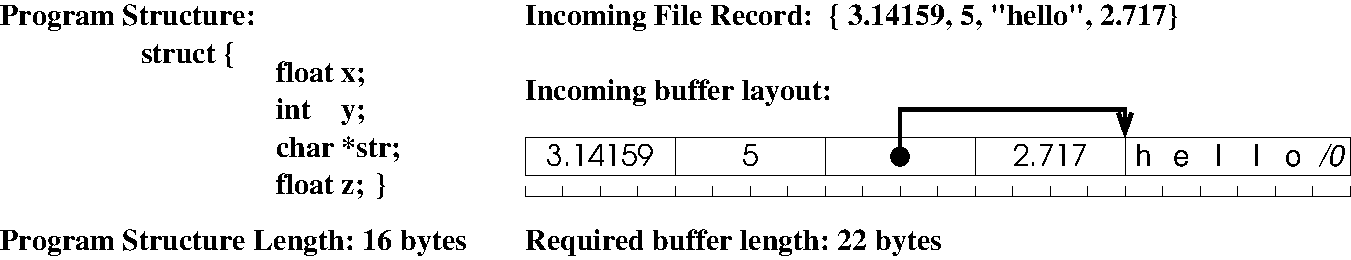
\includegraphics[width=0.7\textwidth]{string_mem.pdf}
\caption{Buffer layout for an incoming record containing a
string.\label{string_mem}} 
\end{center}
\end{figure}
\subsection{Complex Data Types}

PBIO also offers some facilities for constructing records which consist of
more than just the simple data types described in Section~\ref{sec:datatypes}.
The simplest is a mechanism for declaring a field in a record to be an array
of atomic data types.  For example, a type specification of ``integer[5]'' is
understood to be an single dimensional array of 5 integers.  ``float[3][3]''
is a $3\times 3$ two dimensional array floating point numbers.  At present,
PBIO supports these fixed array sizes with one or two dimensions.  The field
size specified should be the size of a single array element, {\bf not} the
size of entire array.  (This convention was different in earlier versions of
this library.)  When reading a record containing array fields, the
dimensionality of each field must match that which was used when the record
was written, though the size of the elements may differ.

It is sometimes useful to use a {\tt \#define}-style constant in array
declarations, but it is awkward to construct the field type string for such
elements because the C preprocessor doesn't expand macros which appear
inside string constants.  To help avoid this awkwardness, the PBIO header
file defines two macros, \routine{IOArrayDecl()} and
\routine{IOArrayDecl2()} that can construct the IOField type string for an
array whose size is fixed by a compile-time constant.  
\begin{figure}[b]
\begin{WrapCode}
#define ARRAY_SIZE 20
#define DIMENSION  30
typedef struct _dyn_rec {
    long        long_value;
    double      double_array[ARRAY_SIZE];
    float      float_array[ARRAY_SIZE];
} rec, *rec_ptr;

IOField rec_field_list[] = {
    {"long_value", "integer", sizeof(long), IOOffset(rec_ptr, icount)},
    {"double_array", IOArrayDecl(float,ARRAY_SIZE), sizeof(double), IOOffset(rec_ptr, double_array)},
    {"float_array", IOArrayDecl2(float,ARRAY_SIZE,DIMENSION), sizeof(float), IOOffset(rec_ptr, float_array)},
    { NULL, NULL, 0, 0}};
\end{WrapCode}
\caption{A record with a compile-time constant as the array size\label{fig:fixarray}}
\end{figure}
For example, the code
in Figure~\ref{fig:fixarray} gives correct PBIO field lists for fixed size
one- and two-dimensional arrays.  For example, the {\tt IOArrayDecl(float,
ARRAY\_SIZE)} macro expanding to the string ``float[20]''.



\begin{wrapfigure}[17]{R}{3.21in}
%\vspace*{-0.25in}
\begin{WrapCode}
typedef struct _dyn_rec {
    char        *string;
    long        icount;
    double      *double_array;
} dyn_rec, *dyn_rec_ptr;

IOField dyn_field_list[] = {
    {"string field", "string", sizeof(char *), 
      IOOffset(dyn_rec_ptr, string)},
    {"icount", "integer", sizeof(long), 
      IOOffset(dyn_rec_ptr, icount)},
    {"double_array", "float[icount]", sizeof(double), 
      IOOffset(dyn_rec_ptr, double_array)},
    { NULL, NULL, 0, 0}
};
\end{WrapCode}
\caption{A dynamic array record format\label{fig:dynarray}}
\index{IOField}
\end{wrapfigure}

In addition to fixed array sizes, PBIO supports dynamically sized
one-dimensional arrays.  In this case, the size in the array type
specification must be the string name of an integer field in the record.
The value of that integer field gives the array size.  The actual data type
in the record should be a pointer to the element type.
Figure~\ref{fig:dynarray} gives an example of a dynamic array declaration.
For the purposes of memory allocation (as discussed in
Section~\ref{stringmem}), the dynamic arrays are treated like strings on
reads.  That is, \routine{read\_IOfile()} leaves the arrays in temporary
memory that will remain valid until the next PBIO operation and
\routine{read\_to\_buffer\_IOfile()} copies the arrays into a user-supplied
buffer.  In the case of a record which contains a dynamic array,
\routine{next\_IOrecord\_length()} still returns the number of bytes
required to hold the entire record including the memory required for the
dynamic array.

\begin{wrapfigure}[5]{R}{2.2in}
\vspace*{-0.25in}
\begin{WrapCode}
 typedef struct R3vector_struct { 
     double x, y, z;
 } R3vector;

 typedef struct particle_struct { 
     R3vector   loc;
     R3vector   deriv1;
     R3vector   deriv2;
 } particle;
\end{WrapCode}
\caption{A nested record format\label{fig:part}}
\index{IOField}
\end{wrapfigure}

Finally, a field type may be the name of a previously registered record
format.  This facility can be used to define record formats in a hierarchical
way.  For example, the structure {\tt particle\_struct} declared as in
Figure~\ref{fig:part} could be written by registering formats defined by these
field lists:
\begin{verbatim}
static IOField R3field_list[] = {
    {"x", "float", sizeof(double), IOOffset(R3vector*, x)},
    {"y", "float", sizeof(double), IOOffset(R3vector*, y)},
    {"z", "float", sizeof(double), IOOffset(R3vector*, z)},
    {NULL, NULL, 0, 0},
};

static IOField particle_field_list[] = {
    {"loc", "R3vector", sizeof(R3vector), IOOffset(particle*, loc)},
    {"deriv1", "R3vector", sizeof(R3vector), IOOffset(particle*, deriv1)},
    {"deriv2", "R3vector", sizeof(R3vector), IOOffset(particle*, deriv2)},
    {NULL, NULL, 0, 0},
};
\end{verbatim}


\subsection{Formats and Record Types}

The programs in Section~\ref{sec:simple} are simplistic in that only known
number records of a single type are written and read.  When multiple formats
or unknown numbers of records are involved, the reading program needs to know
what, if anything, is coming next.  PBIO allows access to this information via
the \routine{next\_IOrecord\_format()} call.  This subroutine returns a value of the
type \routine{IOFormat}.  If this value is NULL, an end of file or error condition has
been encountered.  If non-NULL, the value can be passed to the subroutine
\routine{name\_of\_IOformat()} to get the string name associated with the format of
the next data record.  Additionally, for programs which wish to avoid multiple
string comparison operations on every read operation, PBIO provides the
\routine{get\_IOformat\_by\_name()} subroutine.  With these operations, the simple
reader and writer programs of Section~\ref{sec:simple} can be rewritten to
handle records written in any order.  Figures~\ref{fig:complexwrite}
and~\ref{fig:complexread} give the main bodies of these programs and assume the
structure and field list definitions used earlier in this paper.
\begin{figure}
\begin{WrapCode}
    first_rec_ioformat = register_IOrecord_format("first format", field_list, iofile);
    vec_ioformat = register_IOrecord_format("R3vector", R3field_list, iofile);
    particle_ioformat = register_IOrecord_format("particle", particle_field_list, iofile);
    srandom(time(NULL));
    strcpy(str, "A String");
    rec1.s = str;
    for(i=0; i<10; i++) {
        if (random() % 2 == 1) {
            first_rec rec1;
            rec1.i = i;  rec1.j = 2*i; rec1.d = 2.727 + i; rec1.c = 'A' + 2*i;
            strcat(str, "!");
            if(!write_IOfile(iofile, first_rec_ioformat, &rec1)) {
                printf("write failed\n");
            }
        } else {
            particle p;
            double s = i * i;
            double c = s * i;
            p.deriv2.x = 3.0*i;  p.deriv2.y = 4.2*i;  p.deriv2.z = 4.8*i;
            p.deriv1.x = 1.5*s;  p.deriv1.y = 2.1*s;  p.deriv1.z = 2.4*s;
            p.loc.x    =  .5*c;  p.loc.y    =  .7*c;  p.loc.z    =  .8*c;
            if(!write_IOfile(iofile, particle_ioformat, &p)) {
                printf("write failed\n");
            }
        }
    }
\end{WrapCode}
\caption{The body of a more complex writer program.\label{fig:complexwrite}}
\index{register\_IOrecord\_format()}\index{write\_IOfile}
\end{figure}
\begin{figure}
\begin{Code}
    IOFile iofile = open_IOfile("test_output", "r");
    IOFormat first_format, particle_format, next_format;

    set_IOconversion(iofile, "first format", field_list, sizeof(first_rec));
    set_IOconversion(iofile, "R3vector", R3field_list, sizeof(R3vector));
    set_IOconversion(iofile, "particle", particle_field_list, sizeof(particle));

    first_format = get_IOformat_by_name(iofile, "first format");
    particle_format = get_IOformat_by_name(iofile, "particle");

    next_format = next_IOrecord_format(iofile);
    while(next_format != NULL) {
        if (next_format == first_format) {
            first_rec rec1;
            read_IOfile(iofile, &rec1);
            printf("rec had %d, %d, %g, %s, %c\n", rec1.i, rec1.j, rec1.d, 
                   rec1.s, rec1.c);
        } else if (next_format == particle_format) {
            particle p;
            read_IOfile(iofile, &p);
            printf("particle.loc = %g, %g, %g, deriv1 = %g, %g, %g\n", p.loc.x,
                   p.loc.y, p.loc.z, p.deriv1.x, p.deriv1.y, p.deriv1.z); 
        }
        next_format = next_IOrecord_format(iofile);
    }
\end{Code}
\caption{The body of a more complex reader program.\label{fig:complexread}}
\index{set\_IOconversion()}
\index{next\_IOrecord\_format()}
\index{open\_IOfile()}
\index{get\_IOformat\_by\_name()}
\index{read\_IOfile()}
\end{figure}

The programs in Section~\ref{sec:simple} are also simplistic in that the
writer registers all record formats before writing any data records and the
reader will not work if this condition is violated.  Many simple programs
use a fairly static set of record formats for I/O and have no problems
registering all formats at the beginning.  But in some circumstances,
a program may need to add a new record format at a later time.  Others may
even need to change the layout or sizes of format fields on the fly.  For the
writer, this isn't a significant problem.  PBIO allows new record formats to
be registered to an output stream at any time.  However, reading programs
need a way of knowing when new formats are encountered on input.  

In the PBIO library, data records are just one of the types of records which
appear in the input stream.  Data records are of principal interest to many
programs so the PBIO interface is designed to make access to those records
easy.  However, format descriptions are implicitly written to output streams
whenever a new record format is registered.  In the simple programs presented
thus far, record formats are read implicitly when encountered by the data
input routines.  However, those descriptions are available for reading if so
desired and constitute a second record type.  The current version of PBIO also
allows {\it comments} to be embedded in the data stream.  Comments are simple
null-terminated strings that are not interpreted by the PBIO routines but are
available for ``labeling'' files or data streams.  Comments are written with
the \routine{write\_IOcomment()} function and are the third  type of record which can
appear in  a PBIO input stream.  The function \routine{next\_IOrecord\_type()} returns
the type of the next record in an input stream.  Its return value is one of an
enumeration consisting of the values {\tt \{IOdata, IOformat, IOcomment, IOend,}
and {\tt IOerror\}}.  
\begin{figure}
\begin{verbatim}
    IOFile iofile = open_IOfile("test_output", "r");
    IOFormat first_format, particle_format, next_format;

    while(1) {
        switch(next_IOrecord_type(iofile)) {
        case IOend:
        case IOerror:
            close(iofile);
            exit(0);
            break;
        case IOformat:
            next_format = read_format_IOfile(iofile);
            if (strcmp("first format", name_of_IOformat(next_format)) == 0) {
                first_format = next_format;
                set_IOconversion(iofile, "first format", field_list, sizeof(first_rec));
            } else if (strcmp("particle", name_of_IOformat(next_format)) == 0) {
                particle_format = next_format;
                set_IOconversion(iofile, "particle", particle_field_list, sizeof(particle));
            } else if (strcmp("R3vector", name_of_IOformat(next_format)) == 0) {
                set_IOconversion(iofile, "R3vector", R3field_list, sizeof(R3vector));
            } else {
                /* no need to track other formats */
            }
            break;
        case IOdata:
            next_format = next_IOrecord_format(iofile);
            if (next_format == first_format) {
                first_rec rec1;
                read_IOfile(iofile, &rec1);
                printf("rec had %d, %d, %g, %s, %c\n", rec1.i, rec1.j, rec1.d, 
                       rec1.s, rec1.c);
            } else if (next_format == particle_format) {
                particle p;
                read_IOfile(iofile, &p);
                printf("particle.loc = %g, %g, %g, deriv1 = %g, %g, %g\n", p.loc.x,
                       p.loc.y, p.loc.z, p.deriv1.x, p.deriv1.y, p.deriv1.z); 
            } else {
                /* read and discard other records */
                read_IOfile(iofile, NULL);
            }
            break;
        case IOcomment:
            {
                char *comment = read_comment_IOfile(iofile);
                printf("Got comment >%s<\n", comment);
                break;
            }
        }
    }
\end{verbatim}
\caption{A reader program for dynamic format registration.\label{fig:dynread}}
\index{read\_IOfile()}\index{read\_comment\_IOfile()}\index{open\_IOfile()}
\index{next\_IOrecord\_type()}\index{next\_IOrecord\_format()}
\end{figure}

Figure~\ref{fig:dynread} shows the body of a reader program that is capable of
handling new formats at any time.  Its organization is somewhat different from
the previous reader program of Figure~\ref{fig:complexread}.  For example, the
new program is careful to set conversions for formats only after they have
been read.  Trying to set a conversion for a record format which has not yet
been seen is an error.  The new program also demonstrates how to handle
comments and unwanted records in the input stream.  In the case of comments,
the comment string is held in a buffer internal to PBIO and the
\routine{read\_comment\_IOfile()} call returns a pointer to this buffer.  The buffer
contents are only guaranteed valid until the next PBIO operation.  Unwanted
buffers are discarded by issuing a \routine{read\_IOfile()} call with a NULL buffer
address.  This has the effect of consuming the next buffer on the input
stream.  

\subsection{Bulk Record Handling}

PBIO offers some limited facilities for handling more than one data record at
a time.  These facilities can be separated into two groups, one intended to
support handling contiguous blocks of records and the other for writing smaller
numbers of records.

The support for contiguous blocks of records is provided by the routines:
\begin{verbatim}
extern int
read_array_IOfile(IOFile iofile, void *data, int count, int struct_size);

extern int
write_array_IOfile(IOFile iofile, IOFormat ioformat, void *data, int count, int struct_size);
\end{verbatim}
\routine{write\_array\_IOfile()} writes $count$ records of the same format to the
IOfile.  $data$ points to the start of the block of records and $struct\_size$
must be the size of each array element.  Note that the size of the array
element may be different than the size of the structure outside of the array
because of compiler and data alignment issues.  This type of array write
operation is only available for record formats which do not contain any fields
of type {\tt string}.  All records in the array are written with a single
$write()$ system call.

On the reading side, \routine{read\_array\_IOfile()} performs a similar function.
Records which have been written as arrays can be read individually with the
normal \routine{read\_IOfile()} routine.  However, it is not possible to read as an
array records which have not been written with \routine{write\_array\_IOfile()}.
\routine{read\_array\_IOfile()} returns the number of records which were read, up to
$count$.  All the records will be read with a single $read()$ system call.
The routine \routine{next\_IOrecord\_count()} returns the number of array
records pending.\footnote{``array records'' are records which have been
written with \routine{write\_array\_IOfile()}.  The number pending is the number
remaining in the current set that were written in a single call.}

The other facility for bulk record handling is the routine \routine{writev\_IOfile()}.
\routine{writev\_IOfile()} is similar to the $writev()$ system call.  Instead of taking
single data buffer (of a particular format) to write, \routine{writev\_IOfile()} takes
a list of data buffers and formats.  To the extent possible, all these buffers
will be written to the output stream with a single $writev()$ system
call.\footnote{UNIX typically restricts the number of independent memory areas
that may be written with $writev()$.  If the number and nature of the PBIO
data to be written exceeds this limit, multiple calls will be performed.}
\routine{writev\_IOfile()} imposes no restrictions on the nature of the fields in the
records to be written.  Unfortunately, the nature of the PBIO protocol allows
no corresponding read call.  Records written a single \routine{writev\_IOfile()} must
be read with multiple \routine{read\_IOfile()} calls.  The prototype of
\routine{writev\_IOfile()} is shown in Figure~\ref{fig:writev}.
\begin{figure}[bth]
\begin{verbatim}
typedef struct  pbiovec {
        void    *data;
        IOFormat format;
} *pbiovec;

extern int
writev_IOfile (IOFile iofile, pbiovec vec, int count);
\end{verbatim}
\caption{Prototypes for \routine{writev\_IOfile()}.\label{fig:writev}}
\end{figure}

\subsection{Error Handling}
Most of the routines described in the sections above can detect or return some
kind of error condition.  Some of them are verbose about it, printing error
messages to {\tt stderr}, but most return a particular value when they fail,
generally {\tt NULL} for the routines which return pointers or opaque data
types, like \routine{register\_IOrecord\_format()}, or $0$ for routines like
\routine{read\_IOfile()} which normally return an integer.  Robust programs should
always check the return values of the functions they call.  To facilitate
error handling, PBIO provides two additional functions, {\tt IOhas\_error(IOfile)}
and {\tt IOperror(IOfile, char*)}.  \routine{IOhas\_error()} returns 0 if no error has
occurred on the IOfile specified as its parameter and 1 if an error has
occurred.  \routine{IOperror()} is similar to the UNIX $perror()$ function.  If an
error has occurred on the IOfile specified as its parameter, it prints a
textual message describing the error and includes the string specified as its
second parameter.

\section{Standard Tools for PBIO Files}
The meta-information contained in a PBIO data stream allows the construction
of general tools to operate on PBIO files.  Two such tools are provided with
the PBIO library, IOdump and IOsort.

IOdump is a ``cat'' program for PBIO files.  IOdump takes as arguments a set
of options and a filename.  By default IOdump prints an ascii representation
of all data records and comments in the PBIO file.  Dumping of record format
information as well as header information in the file is enabled by specifying
options of {\tt +formats} and {\tt +header} respectively.  In general,
printing for any record type can be turned on or off by specifying options
of the form {\tt \{+,-\}\{header, comments, formats, data\}}.

IOsort is a generalized sorting program for PBIO files.  It takes three
parameters, the name of the field to sort upon, the name of the input file and
the name of the output file.  The sort field can be of any PBIO atomic data
type, but it must be the same basic type in all records.  Any records in which
the sort field does not appear will not appear in the output file.

\section{PBIO With Other Networks}

The basic PBIO routines above provide for using PBIO for I/O over file
descriptors.  This is sufficient for normal file and TCP/IP socket uses.  But
sometimes it is useful to use PBIO in other network circumstances as well.
PBIO contains two types of support for transmission over networks without
using a TCP/IP layer.  The first type of support is designed for networks
which still provide a TCP-like reliable, in-order, two-ended connection.  The
second provides a broader kind of support which makes no assumptions about the
underlying network.

\subsection{Customizing PBIO Low-Level I/O}

To support binary I/O over networks providing a TCP-like interface, PBIO
allows the substitution of user-supplied low-level I/O routines for those
normally used to operate on the network interface.  To support the full range
of PBIO operations, the user must supply routines to read and write the
network interface, a function to poll the network interface for new data and a
routine to close the network interface.  A typical call sequence to create a
new PBIO file with a different low-level I/O interface follows:

\begin{Code}
{
    IOFile iofile = create_IOfile();  /* initialize IOfile structure */
    void *conn_info;
    /*
     * user code to create a network connection.  Upon creation,
     * place any information necessary to use the connection in
     * conn_info.  This pointer will be supplied to the read and 
     * write routines.
     */
    set_fd_IOfile(iofile, conn_info);  /* assoc net info with iofile */

    set_interface_IOfile(iofile, new_write_func, new_read_func,
                         new_writev_func, new_readv_func, new_max_iov,
                         new_close_func, new_poll_func);

    open_created_IOfile(iofile, "w");  /* open file for writing */

    /* after this, operate on iofile with normal calls */
}
\end{Code}
\index{set\_fd\_IOfile()}\index{set\_interface\_IOfile()}\index{open\_created\_IOfile()}
\sloppy In the code above, the six functions {\tt new\_write\_func},
{\tt new\_read\_func}, {\tt new\_writev\_func}, {\tt new\_readv\_func}, {\tt
new\_close\_func} and
{\tt new\_poll\_func} are the new user-supplied network access routines.  {\tt
new\_write\_func} and {\tt new\_read\_func} are both of type {\tt
IOinterface\_func} as defined in io\_interface.h:
\begin{Code}
typedef int (*IOinterface_func)(void *conn, void *buffer, int length,
                                int *errno_p, char **result_p);
\end{Code}
When PBIO calls these routines, the value used in the \routine{set\_fd\_IOfile()}
call will be supplied as the {\tt conn} parameter.  {\tt buffer} and  {\tt
length} specify the buffer to be read or written.  Upon correct completion,
the routines should return the number of bytes read or written.  In the event
of end of file, the function should return 0.  In the event of other error,
the {\tt errno\_p} or {\tt result\_p} parameters are used to specify the nature
of the error.  If the error is one which maps to a standard UNIX errno value,
the integer pointed to by errno\_p should be set to that value.  If not, the
{\tt char*} pointed to by {\tt result\_p} should be set to a string describing
the error.  (This string will not be free()'d by PBIO.  If it is not stored
in static memory, the user routines should ensure that it is deallocated.)

The routines {\tt new\_readv\_func} and {\tt new\_writev\_func} are called by
PBIO to read or write multiple buffers at a time.  They are of type {\tt
IOinterface\_funcv}:
\begin{Code}
typedef int (*IOinterface_funcv)(void *conn, struct iovec *iov, int icount,
                                 int *errno_p, char **result_p);
\end{Code}
They are like the read and write functions except that instead of a single
buffer and length, they take a vector of type {\tt struct iovec} and a buffer
count value. Type {struct iovec} is an address,length pair.  If the network
interface imposes a maximum size on the number of buffers which can be
efficiently read or written in one call, that value should be specified as the
{\tt max\_iov} value in the \routine{set\_interface\_IOfile()} call.  If the
network interface provides no direct multi-buffer read or write primitives,
the readv and writev functions can be specified as NULL.  In this case, PBIO
will instead generate multiple calls to the single-buffer read and write
routines. 

The {\tt new\_close\_func} and {\tt new\_poll\_func} routines each take only
the {\tt void *conn} value as a parameter.  The close function should shut
down the network connection and free all resources associated with it.  Poll
should return zero if there is no data currently available for reading on the
network interface.  PBIO does not use this function except in the routine
\routine{poll\_IOfile()}.  Consequently, if the network interface does not
provide any 
means of polling the network for data, this function can possibly be left NULL
with no ill effects.  If \routine{poll\_IOfile()} is called when the poll function
is NULL, \routine{poll\_IOfile()} arbitrarily returns 0 (I.E. no data pending).

\subsection{PBIO with Arbitrary Networks\label{iocontext}}

There are many network transport mechanisms which are not TCP/IP-like in one
way or another.  Some relax reliability or ordering characteristics to achieve
higher performance.  Others vary topology to support such things as multiple
receivers (broadcast and multicast) or multiple senders (with incoming
messages multiplexed over a single connection).  Different applications may
choose to use one of these network protocols for the actual transport of data
but would still find it useful to use PBIO to handle the heterogeneity issues.
Unfortunately, it is difficult for PBIO to deal directly with a
non-TCP/IP-like network interface.  In particular, the basic PBIO functions
assume that the input appearing at the ``read'' port of an IOfile should be
exactly what is written from the ``write'' side of a single IOfile.  This is a
natural assumption for TCP/IP like transports, but it breaks down if the
underlying transport mechanism allows multiplexing of writers or readers or if
it does not guarantee reliable, in-order delivery.  PBIO could theoretically
tolerate the loss or misordering of complete data records, but multiplexing of
streams, delivery partial data records or any disruption affecting record
format information would render some data uninterpretable. 

In order to allow applications to gain the functional benefits of PBIO while
using network transport mechanisms which PBIO can not directly support, we
have defined an interface that allows separating the processes of data
transport and format delivery.  With this interface, instead of using
\routine{write\_IOfile()} to transmit data, applications can {\em encode} the data in
a form that can be interpreted by another PBIO library.  The application can
then transmitted this encoded buffer via any mechanism at its disposal.  Once
at its destination, the encoded buffer can then be passed to PBIO for decoding.
Throughout this process, the transmission of format information from the
encoder to the decoder is handled transparently by PBIO.  Formats still need
to be registered on the encoding side and conversions need to be set on the
decoding side, but record format information travels from the encoder to the
decoder via private reliable connections established by PBIO.
Section~\ref{sec:formats} will discuss format communication in more detail.

The programs below show a simple use of these functions to transfer data.
Here, the data is encoded in one program, ``transmitted'' by writing it to a
file in one program and reading it in another,\footnote{Of course, storing
data in a file is the normal function of the \{read,write\}\_IOfile
interface.  Files are used here only as an example transport mechanism.}
and finally decoded in the ``receiving'' program.  
\label{contextcode}
\begin{Code}
void main()     /* sending program */
{
    IOContext src_context = create_IOcontext();
    IOFormat dyn_rec_ioformat;
    dyn_rec rec;
    int buf_size, fd, i;
    char *encoded_buffer;
    dyn_rec_ioformat = register_IOcontext_format("dynamic format",
                                                  dyn_field_list,
                                                  src_context);
    rec.string = "Hi Mom!";
    rec.icount = 5;
    rec.double_array = (double*) malloc(sizeof(double) * 5);
    for (i=0; i<5; i++) 
        rec.double_array[i] = i*2.717;
    encoded_buffer = encode_IOcontext_buffer(src_context, 
                        dyn_rec_ioformat, &rec, &buf_size);

    /* "transmit" encoded record over a file */
    fd = open("enc_file", O_WRONLY|O_CREAT|O_TRUNC, 0777);
    write(fd, encoded_buffer, buf_size);
}
\end{Code}
\index{create\_IOcontext()}\index{register\_IOcontext\_format()}\index{encode\_IOcontext\_buffer()}
\begin{Code}
void main()     /* receiving program */
{
    IOContext dest_context = create_IOcontext();
    IOFormat dyn_rec_ioformat;
    dyn_rec rec;
    int fd, i;
    char encoded_buffer[2048];  /* hopefully big enough */

    /* "receive" encoded record over a file */
    fd = open("enc_file", O_RDONLY, 0777);
    read(fd, encoded_buffer, sizeof(encoded_buffer));

    dyn_rec_ioformat = get_format_IOcontext(dest_context, encoded_buffer);
    set_conversion_IOcontext(dest_context, dyn_rec_ioformat,
                             dyn_field_list, sizeof(dyn_rec));
    decode_IOcontext(dest_context, encoded_buffer, &rec);
    printf("string is %s\n", rec.string);
    printf("icount is %d\n", rec.icount);
    for(i=0; i< rec.icount; i++)
        printf("element %d is %g\n", i, rec.double_array[i]);
}
\end{Code}
\index{create\_IOcontext()}\index{get\_format\_IOcontext()}\index{decode\_IOcontext()}
The example programs above are quite simple, but they illustrate two basic
characteristics of the IOContext interface:
\begin{itemize}
\item record formats and conversions are registered and set in an \routine{IOContext} value, much as they are in \routine{IOFile}'s in the connected
interface.  However, unlike the \routine{IOFile}, the \routine{IOContext} is not
directly associated with a file, socket or other transmission or storage
mechanism.  It only serves as a placeholder to hold registration and
conversion information.
\item The example uses files as a ``transport'' mechanism, but PBIO isn't
involved in the movement of the encoded data.  Actual transmission from
encoder to decoder could be via TCP, UDP or paper-tape clutched by a carrier
pigeon.  All that matters to PBIO is that the block of data presented to
\routine{decode\_IOcontext()} must be one that resulted from a call to
\routine{encode\_IOcontext()}.
\end{itemize}

The extreme simplicity of the examples allows the omission of details that
would complicate the logic of more general programs.  For example:
\begin{itemize}
\item The receiving program sets a conversion for the record without examining
its format, implicitly assuming that it is a format that can be converted to
the type {\tt dyn\_rec}.  A complex program supporting multiple record
formats would presumably examine at least the name and perhaps the fields of
the format before deciding which conversion to register for it.  The function
\routine{has\_conversion\_IOformat()} returns true if a
conversion has already been registered for a particular format, false
otherwise. 
\item Additionally, to support record formats which might have nested
subformats such as the record described in Figure~\ref{fig:part}, the use of
an additional functions.  In particular, \routine{get\_format\_IOcontext()}
returns only the top-level format of the record.  But conversions must be set
for any nested formats before a top-level conversion can be set.  The PBIO
routine \routine{get\_subformats\_IOcontext()} (prototype below) returns a
NULL-terminated list of IOFormat values corresponding to any nested formats
contained within the record.  The last entry in the list is the format of the
record itself.  The format list returned by this function should be free'd
when no longer needed.
\ \begin{Code}
extern IOFormat *get_subformats_IOcontext(IOContext iocontext, void *buffer);
\end{Code}
\index{get\_subformats\_IOcontext()}

\item Because the examples just exchange a single record, they do not need to
explicitly mark the beginning or end of the encoded data blocks.  Because
attempting to decode an incomplete or corrupted data block is likely to have
unpredictable and deleterious consequences, applications should take steps to
ensure that the data blocks they decode are always the complete and
uncorrupted result of some encode operation.
\item The examples each use a single IOContext and use it for a single
operation.  Individual IOcontext values can be used for both encoding and
decoding and those operations will not affect each other.  Many applications
can get by with a single IOContext value per process, but more may be used to
accommodate different threads of control or to ease management of the temporary
memory provided by IOcontexts.
\end{itemize}

\subsubsection{Memory Handling in the IOContext Interface}

As with the IOFile interface, the memory use characteristics of the IOContext
interface require documentation.  

\paragraph{Transmitting/encoding side}
On the encoding side, the encoded data block is stored in temporary memory
internal to PBIO and specific to the IOContext value used to encode the data.
The memory will remain valid until the next encode or decode operation
associated with that IOContext value.  

In addition to the basic \routine{encode\_IOcontext\_buffer()} routine,
there are several other variations that manage their encoding differently
and which may be more advantageous to use in certain circumstances.  For
example, the routine \routine{encode\_IOcontext\_bufferB()} encodes into a
contiguous memory block, but instead of using temporary memory associated
with the \routine{IOContext}, it uses memory associated with an
\routine{IOBuffer} variable.  \routine{IOBuffer}s exist solely as a handle
to temporary memory space that can be used by PBIO.  Using memory associated
with an \routine{IOBuffer} instead of an \routine{IOContext} decouples the
memory use from the IOcontext so that a following encode does not
automatically destroy the data in memory occupied by a prior encode.
\routine{IOBuffer}s are allocated with \routine{create\_IOBuffer()} and
destroyed with \routine{free\_IOBuffer()}.  Note that the pointer returned
by \routine{encode\_IOcontext\_bufferB()} should not be free'd.  That memory
will be deallocated when the \routine{IOBuffer} is free'd.
\routine{IOBuffer}s may be used multiple times before they are deallocated,
with the caveat that each reuse destroys the previous contents.
The APIs for these routines are:
\begin{WrapCode}
extern IOBuffer create_IOBuffer();
extern void free_IOBuffer(IOBuffer buf);
extern char *encode_IOcontext_bufferB(IOContext iocontext, IOFormat ioformat, IOBuffer iobuffer, 
                                      void *data, int *buf_size);
\end{WrapCode}

Two additional variations of the PBIO encode routines are
\routine{encode\_IOcontext\_to\_vector()} and
\routine{encode\_IOcontext\_to\_vectorB()}.  The vector-based encode can be
somewhat more efficient than the routines that return a contiguous block of
encoded data because the contiguous-buffer routines necessarily copy all of
the data from its original location to the final buffer.  Since PBIO tries
to transmit all data in its original representation, some copy overhead can
be eliminated by representing the return value from an encode operation as a
list of memory blocks to be transmitted, rather than a single contiguous
block.  In that list of memory blocks, some blocks will be segments of 
temporary memory and some will be components of the original data.
If whatever message transport mechanism is being used requires a contiguous
block of data, it is best to use the {\tt encode\_IOcontext\_buffer()}
routines.  But if the transport can handle lists of buffers, such as the
Unix-style {\tt writev()} call, copy elimination can significantly improve
performance where large data blocks are involved.  For example, the encoding
example above can be rewritten to use the vector based calls as seem below:
\begin{Code}
void main()     /* sending program */
{
    IOContext src_context = create_IOcontext();
    IOFormat dyn_rec_ioformat;
    dyn_rec rec;
    int iovcnt, fd, i;
    IOEncodeVector encode_vector;
    dyn_rec_ioformat = register_IOcontext_format("dynamic format",
                                                  dyn_field_list,
                                                  src_context);
    rec.string = "Hi Mom!";
    rec.icount = 5;
    rec.double_array = (double*) malloc(sizeof(double) * 5);
    for (i=0; i<5; i++) 
        rec.double_array[i] = i*2.717;
    encoode_vector = encode_IOcontext_to_vector(src_context, 
                        dyn_rec_ioformat, &rec);

    /* count the number of blocks */
    iovcnt = 0;
    while (encode_vector[iovcnt].iov_base != NULL) iovcnt++;

    /* "transmit" encoded record over a file */
    fd = open("enc_file", O_WRONLY|O_CREAT|O_TRUNC, 0777);
    writev(fd, encode_vector, iovcnt);
}
\end{Code}
\index{create\_IOcontext()}\index{register\_IOcontext\_format()}\index{encode\_IOcontext\_to\_vector()}
The full APIs of the vector-based encoding routines are given below.  As in
the buffer-based routines, there is a version that uses an
\routine{IOBuffer} variable to supply the temporary memory necessary for the
encoding. 
\begin{WrapCode}
typedef struct _io_encode_vec {
     void *iov_base;
     long  iov_len;
} *IOEncodeVector;

extern IOEncodeVector
encode_IOcontext_to_vector(IOContext iocontext, IOFormat ioformat, void *data);

extern IOEncodeVector
encode_IOcontext_vectorB(IOContext iocontext, IOBuffer tmp_buffer, IOFormat ioformat, void *data);
\end{WrapCode}

\paragraph{Receiving/decoding side}
On the receiving end, PBIO offers three different decode operations.  The
operations \routine{decode\_IOcontext()} and \routine{decode\_to\_buffer\_IOcontext()}
are analogous to \routine{read\_IOfile()} and \routine{read\_to\_buffer\_IOfile()}.
In both cases, the encoded data is preserved and the base record structure
(excluding strings and dynamic arrays) in placed in memory provided by the
user.  In \routine{decode\_IOcontext()} (as in \routine{read\_IOfile()}), strings and
dynamic arrays are copied into PBIO temporary memory associated with the
decoding IOContext.  The contents of that memory will remain valid until the
next encode or decode operation performed in that context.  However, in
\routine{decode\_to\_buffer\_IOcontext()}, all data is placed in
user-supplied memory. 
The routine:
\begin{Code}
extern int
this_IOrecord_length(IOContext context, char *src, int encoded_record_length);
\end{Code}
\index{this\_IOrecord\_length()}
returns the number of bytes of user memory required to hold the decoded record.
This call requires the length of the encoded record block as a parameter and
returns a conservative estimate of the number of bytes required to decode the
record.  

The third decode option offered by PBIO is
\routine{decode\_in\_place\_IOcontext()}.  The first two calls,
\routine{decode\_IOcontext()} and \routine{decode\_to\_buffer\_IOcontext()},
always leave 
their output in a different location than where the encoded buffer resides.
This requires even data fields that need no significant modification to be
moved to a different location and may not the most efficient way to decode the
record.  This is particularly true for transfers between homogeneous targets.
In contrast, \routine{decode\_in\_place\_IOcontext()} attempts to decode the
message and leave it where it is in memory.  Where this is possible it is at
least as efficient as \routine{decode\_IOcontext()} and perhaps much more
efficient because it need not involve any significant data movement.  However,
sometimes it isn't possible to decode the buffer in place.  Sometimes the
fields in the current and the desired structure overlap in ways that make it
difficult to rearrange them in place.  When this kind of conflict happens,
\routine{decode\_in\_place\_IOcontext()} must copy the encoded buffer into a
temporary location (managed by PBIO), and then do a normal
\routine{decode\_IOcontext()} with the source being the temporary buffer and
the 
destination being where the data used to sit.

Despite differences in performance, each call will always maintain the
appropriate semantics.
That is, \routine{decode\_in\_place\_IOcontext()} will always leave the result in
the same memory as the encoded buffer and \routine{decode\_IOcontext()} will
always leave the result in the specified destination buffer.  Some programs
may choose to ignore the performance differences and use one call or the other
depending upon which of those semantics best fits the memory use requirements
of the application.  However, smarter applications can achieve the best of
both worlds by making use of the \routine{decode\_in\_place\_possible()} routine
which separates the two possible situations.  The following example
demonstrates its use.
\begin{Code}
    /* buffer msg contains encoded message */
    IOFormat format = get_format_IOcontext(context, msg);

    if (decode_in_place_possible(format)) {
        char *msg_start;
        decode_in_place_IOcontext(context, msg, &msg_start);
        /*
         * note that with an in-place decode, byte 0 of the resulting
         * decoded structure is probably not at byte 0 of the encoded
         * buffer.  Therefore, msg_start is probably a few bytes into
         * the buffer msg.  The precise relationship between msg and
         * msg_start is a PBIO implementation detail.
         */
        process_message(msg_start);
    } else {
        int length = this_IOrecord_length(context, msg, incoming_size);
        char *new_msg = malloc(length);
        decode_to_buffer_IOcontext(context, msg, new_msg);
        process_message(new_msg);
        free(new_msg);
    }

\end{Code}
\subsubsection{Communication of Format Information\label{sec:formats}}
While the actual communication of record format information from the
encoding context to the decoding context is generally handled entirely
within PBIO, the manner in which this communication is accomplished may
influence the behavior of the application in some ways.

PBIO does have mechanisms and APIs through which applications can directly
participate and manage the exchange of format information.  However, those
mechanisms are complex and their use is a topic beyond the bounds of this
manual.  Therefore we describe the one standard mechanism for managing
format informat, the use of a third party {\it format server}.  When a
\routine{register\_IOcontext\_format()} is done, PBIO synchronously and
reliably transmits record format information to a {\it format server},
running on a known host and listening at a known port.  Then, PBIO waits for
the format server to return to it a 64-bit format ID.  The
\routine{register\_IOcontext\_format()} operation returns only when the
format ID has been received at the encoding side and stored with the
IOContext value.  When data for that format is encoded, PBIO appends the
format ID to the data to identify the format.  On the receiving side,
\routine{get\_format\_IOcontext()} extracts the 64-bit format ID from the
data and looks in the decoding IOContext to see if that particular format ID
has been seen before.  If not, PBIO synchronously queries the format server
and retrieves the format of record.  Thereafter, the format information is
associated with the format ID in the IOContext value and no further contact
with the format server is necessary to process records of this
type.\footnote{However, as this association is maintained in the IOContext
value, the use of multiple IOContexts may require multiple contacts to the
format server.}

The use of a centralized format server as a data repository has several side
effects.  As a centralized resource, the format server is a possible
bottleneck in a large system.  To mitigate this effect, the format server
consolidates identical record formats registered by hosts of the same
architecture and assigns them all the same format ID.  This means that a
host receiving the same type of information from $N$ machines of $M$
different types will only query the format server $M$ times.  Another side
effect is that the format server is subject to periodic information loss due
to power outages, etc.  This possibility limits the length of time a format
ID will remain associated with a particular set of format information, and
may potentially limit the life of encoded data.  Because events that require
a format server to restart are rare in practice, because many applications
that exchange data online are relatively short lived, and because 
the IOFile() interface is available for long-term data storage, most
applications are not affected in any way by the robustness of the format
server.  For those applications that may be especially long-lived, the
format server does have a checkpoint/restart mechanism that allows format
IDs to remain valid across multiple server instances.

At this time the location (host and IP port) of the format server is a
compile-time parameter to PBIO.  The host value in particular is encoded in
the file \routine{config.h} by the \routine{configure} script.  The
actual value placed in \routine{config.h} is controlled by the optional {\tt
--with-format-server=HOST} argument to {\tt configure}.  
\index{configure!--with-format-server}
If this argument is specified at build time, it is used as the default host
for the PBIO library to attempt to contact a format server.  If that
argument is not specified at build time, the default format server host will
be the host upon which the configure script is running.\footnote{Except when
the script is running in the ``gatech.edu'' network domain.  Then the
default format server host will be marquesas.cc.gatech.edu.}  The format
server host which was specified at build time for the PBIO library may be
overridden at run-time through the use of the \routine{FORMAT\_SERVER\_HOST}
environment variable.\index{environment variables!FORMAT\_SERVER\_HOST}

If no format server responds at the default host, PBIO will attempt to
contact a ``fallback'' format server.  At the present time, this is always
the format server on marquesas.cc.gatech.edu.  Because we don't want the
format server on marquesas to be the default server for the world, there is
a primitive protection mechanism built into the format server.  In
particular, the format server has a {\it format service domain} build
parameter.  When a client connects to a format server, the server uses a
reverse DNS lookup based on the peer IP address associated with the
connection to determine the clients hostname.  If the hostname appears to be
within the {\it format service domain}, the client is allowed unconditional
access to the format server.  However, if the hostname is outside of the
domain, or if the hostname lookup fails, the IP address of that client is
logged and clients from that IP address may only use the format server for
three (3) days.  The client will print a provisional use warning that states
the ``contacted format\_server daemon allows only temporary
use.''\index{format server!temporary use}  Connections from IP addresses
that have expired will be rejected.  The list of expired IP address is 
{\it not} part of the checkpoint/restore format server functionality, so
restarting the format server will reset the list to empty.  The actual
service domain used is a build-time parameter to PBIO and is controlled by
the the optional {\tt --with-service-domain=DOMAINLIST} argument to {\tt
configure}.\index{configure!--with-service-domain}  DOMAINLIST is a list of
domain names separated with ':' characters.  If the argument is not given,
the DOMAINLIST defaults to empty, which allows unrestricted access to all
hosts.\footnote{Except when the configure scripts is run on machines in the
gatech.edu domain.  In this case the default DOMAINLIST is
``gt.atl.ga.us:gatech.edu''.} 


\section{XML and PBIO/JIX\label{XML}}

PBIO's XML support had its origins in the observation that PBIO and XML both
provide similar semantics to the receivers of data.  Both formats are
self-describing and allow third-parties to interpret and process data about
which they have no {\it a priori} knowledge.  Both formats also allow
readers to be relatively robust to changes in the data that is sent.  In
particular, most mechanisms for reading XML (parsers, DOM interfaces, etc.)
do not depend upon the ordering of fields in the XML document and are not
affected if the XML document contains extra fields are attributes.  PBIO is
similar because of the semantics of the \routine{set\_IOConversion()} and
\routine{set\_conversion\_IOcontext()} routines.  In particular, the
\routine{IOFieldList} supplied in the conversion call specifies the order
and layout that the receiver want to see the data in.  If the incoming data
contains fields in a different order or contains additional fields, those
differences are resolved in the conversion process.  Fields are reordered
and extraneous fields are dropped.

\subsection{Operating on Unknown Data}
Our experience with PBIO has shown that most programs do not operate upon
data that they have no prior knowledge about.  While PBIO
\routine{IOFieldList}s can be created and used dynamically, it is a rare
practice because it is only necessary if the structures to be manipulated
are dynamic and that is not a semantic that is directly supported by common
programming environments.  Therefore, PBIOs routines that query and
manipulate field lists will not be described in detail here.  Instead we
will just enumerate them below:
\begin{description}
\item[{\tt extern IOFieldList field\_list\_of\_IOformat(IOFormat format)}]
returns the NULL-terminated \routine{IOFieldList} associated with a given
\index{field\_list\_of\_IOformat()}
\item[{\tt extern int compare\_field\_lists(IOFieldList list1, IOFieldList
list2)}]
compares two field lists for strict equality.
\index{compare\_field\_lists()}
\item[{\tt extern IOFieldList copy\_field\_list(IOFieldList list)}]
returns a copy of an {\tt IOFieldList}
\index{copy\_field\_list()}
\item[{\tt extern IOFieldList localize\_field\_list(IOFieldList list)}]
this routine assigns ``reasonable'' values to the size and offset values
for the given field list.  Here ``reasonable'' means acceptable to the
current underlying machine architecture.  This routine is used to support
higher-level dynamic code generation routines in doing third-party data
processing and filtering.
\index{localize\_field\_list()}
\item[{\tt extern int struct\_size\_field\_list(IOFieldList list, int pointer\_size)}]
returns the size of the ``base'' structure described by a field list.  The
{\tt pointer\_size} parameter is required because that information is
implicit in format registration and not carried with the field list.
\index{struct\_size\_field\_list()}
\end{description}

\subsection{Just-In-Time Expansion to XML}

Because PBIO records are completely self-describing, it is possible to
``print'' them into XML (or virtually any ASCII form) at any point.  Two
subroutines in PBIO specifically support the production of XML.  One,
\routine{IOencoded\_to\_XML\_string()} operates on data in its encoded form
(as produced by \routine{encode\_IOcontext\_buffer()} for example).  The
second, \routine{IOunencoded\_to\_XML\_string()} operates on unencoded data.
Both routines return a {\tt char*} string value that is the XML
representation of the data.  The string should be {\tt free}'d when it is no
longer needed.  The APIs of these routines are:
\begin{WrapCode}
extern char *IOencoded_to_XML_string(IOContext iocontext, void *data);

extern char *IOunencoded_to_XML_string(IOContext iocontext, IOFormat ioformat, void *data));
\end{WrapCode}
By default, the XML expansion of PBIO data is relatively simple and is
governed by the format that describes the data.  The
``format\_name'' string provided in the original
\routine{register\_IOcontext\_format()} call is used as the name in the
surrounding begin/end XML tags for a structure.  Within a structure, each
fields name is used in begin/end XML tags for that field.  Within the field
begin/end tags is XML that represents the contents of that field.  If the
field type is a simple atomic type, the contents are simply printed in an
appropriate format.  Integer types appear in decimal representations,
characters as simple chars, booleans appear as either ``true'' or ``false'',
strings appear directly and floating point types are printed using the
``%g'' representation provided by the system's C library.  Nested structures
appear as nested XML elements.  Arrays appear as repeated XML elements.  In
arrays of atomic data types, the field name appears as the standard
begin/end XML tags where the element contents are the actual array element
values with whitespace separators.  Fixed-length and variable-length arrays
are treated identically.

For example, the record written in the simple encoding example of
Section~\ref{contextcode} expands to the following XML if
\routine{IOencoded\_to\_XML\_string()} is called on the resulting encoded
buffer. 
\begin{verbatim}
<dynamic format>
<string field>Hi Mom!</string field>
<icount>5</icount>
<double_array>
0 2.717 5.434 8.151 10.868 </double_array>
</dynamic format>
\end{verbatim}

\subsection{Customizing the XML Representation}
Note that in the default XML representation, all data is presented as an XML
element without use of XML attributes.  In practice, users may require more
control of the manner in which PBIO-based records are expanded as XML.
In PBIO's model of XML support, additional XML markup information can be
associated with \routine{IOFormat}s at the time of
registration.\footnote{Note that this approach means that XML formatting is
controlled at the time of encoding of data, not at the point at which it is
hydrated into XML.}  The mechanism for this is a special format registration
call that allows {\it optional} format information to be specified along
with the registration.  The optional format information API is generalized
for future extensions, though at the time of this writing the only optional
information supported is the XML markup information.\index{format
registration!optional information}  The API for registering a format with
optional information and for retrieving the optional information associated
with a format is shown below:
\index{IOOptInfo}\index{register\_opt\_format()}\index{get\_optinfo\_IOformat()}
\begin{Code}
typedef struct _IOOptInfo {
    int info_type;
    int info_len;
    char *info_block;
} IOOptInfo;

extern IOFormat register_opt_format(const char *format_name, IOFieldList field_list,
				    IOOptInfo *optinfo, IOContext iocontext);
extern void * get_optinfo_IOFormat(IOFormat ioformat, int info_type, int *len_p);
\end{Code}
The {\tt optinfo} parameter to \routine{register\_opt\_format()} is a list
of optional information values to be associated with the format.  The list
is terminated by an entry with an {\tt info\_type} value of 0.  To specify
optional XML markup information, the {\tt info\_type} value must be {\tt
XML\_OPT\_INFO}, the {\tt info\_block} value should point to an XML markup
string, and the {\tt info\_len} parameter should be set to the length of the
markup string.  The format of the markup string is described in the next
sections.

\subsubsection{Basic XML Markup}
The XML markup string is essentially a template into which the values from
the actual data will be substituted.  The substitution points are marked by
XML-like {\tt PBIO:data} tags.  Those tags contain as an attribute the
identity of the particular data field that is to be substituted, specified
by either {\tt field\_name} or {\tt field\_id} (a zero-based index into the
field list).  Except for {\tt PBIO:*} tags, {\it all} elements of the XML
markup string are copied directly from the template into the hydrated XML.
Thus, any non-variant elements in the XML, including tags, constant
attributes, or whitespace, can be supplied with the XML markup.  For example,
an XML markup string that will produce exactly the default output for the
example above is:
\begin{verbatim}
"<dynamic format>
<string field><PBIO:data field_name="string field"></string field>
<icount><PBIO:data field_name=icount></icount>
<double_array>
<PBIO:data field_id=2></double_array>
</dynamic format>"
\end{verbatim}
Note the variations in the attribute associated with each {\tt PBIO:data}
tag.  Field names are used for the first two tags, and in the case of {\tt
string field} the name must be surrounded by quotes because it contains a
space character.  The last field is specified by its zero-based index in the
field list (``double\_array'' is field 2).


\begin{verbatim}
"<?xml version="1.0" encoding="ISO-8859-1"?>
<!DOCTYPE dynamic [
        <!ELEMENT dynamic (strfield, icount, doublearray)>
        <!ELEMENT strfield (#PCDATA)>
        <!ELEMENT icount (#PCDATA)>
        <!ELEMENT doublearray (#PCDATA)>
]>
<dynamic>
        <strfield><PBIO:data field_name="string field"></strfield>
        <icount><PBIO:data field_name=icount></icount>
        <doublearray><PBIO:data field_name=double_array></doublearray>
</dynamic>"
\end{verbatim}
A program that demonstrates this facility and its output appear in
Figures~\ref{xml_fig} and \ref{xml_output}.
\begin{figure}[p]
\begin{quote}
\VerbatimInput{manual_test.c}
\end{quote}
\caption{A program using explicit XML markup specified as optional
information in format registration.\label{xml_fig}}
\end{figure}
\begin{figure}[t]
\begin{quote}
\VerbatimInput{xml_output}
\end{quote}
\caption{Output for the program in the previous figure.\label{xml_output}}
\end{figure}
\subsubsection{XML Markup for Arrays}
The simple template mechanism discussed is perfectly adequate for simple
and nested structures, but doesn't allow complete control of how arrays are
hydrated into XML.  In particular, the use of a simple {\tt PBIO:data} tag
doesn't allow control of the text that is to appear before and after each
array element.  In order to attain that control, we again follow an XML
style in the template and introduce two new tags, {\tt PBIO:array} and {\tt
PBIO:array\_data\_mark}.  Essentially, where the basic use of {\tt PBIO:data}
produces a template with this conceptual behavior:
\begin{quote}
\small
$\dots${\tt <PBIO:data field\_name=field\_a>}\\
{\it text between field\_a and field\_b (appears once)}\\
{\tt <PBIO:data field\_name=field\_b>}\\
{\it text between field\_b and field\_c> (appears once)}\\
{\tt <PBIO:data field\_name=field\_c>}
$\dots$
\end{quote}
The new tags define the text in this manner:
\begin{quote}
\small
$\dots${\tt <PBIO:data field\_name=field\_a>}\\
{\it text between field\_a and start of array (appears once)}\\
{\tt <PBIO:array>}\\
{\it text that appears before every array element}\\
{\tt <PBIO:array\_data\_tag field\_name=field\_b>}\\
{\it text that appears after every array element}\\
{\tt </PBIO:array>}\\
{\it text after array and before field\_c (appears once)}\\
{\tt <PBIO:data field\_name=field\_c>}
$\dots$
\end{quote}
This is sufficient to allow complete control if the representation of arrays in
lists in XML hydration.  As an example of using this facility, consider the
program of Figure~\ref{xml_fig} and replace the line ``{\tt
<doublearray><PBIO:data field\_name=double\_array></doublearray>}'' with:
\begin{Code}
	<doublearray><PBIO:array>
	    <list_element>
		<PBIO:array_data_mark field_name=double_array>
	    </list_element></PBIO:array>
	</doublearray>
\end{Code}
The modified portion of the  output of the program is shown in Figure~\ref{xml_output2}.
\begin{figure}[t]
\VerbatimInput{xml_output2}
\caption{New output with array expansion explicitly controlled.\label{xml_output2}}
\end{figure}

\section{Statistical Information}
\begin{wrapfigure}[10]{R}{3.5in}
\vspace*{-.5in}
\begin{WrapCode}
struct _IOContext_stats {
    int decode_bytes;
    int decode_msg_count;
    int encode_bytes;
    int encode_msg_count;
    int formats_present_count;
    int format_registration_count;
    int format_fetch_count;
    int to_format_server_bytes;
    int from_format_server_bytes;
    long last_server_time;
} *IOContext_stats;
extern IOContext_stats get_IOstats(IOContext iocontext);
extern void print_IOstats(IOContext_stats);
\end{WrapCode}
\end{wrapfigure}
The library does track some basic information relating to basic input and
output statistics.  The tracking is centered on \routine{IOContext}s and
\routine{IOFile}s and is available with the \routine{get\_IOstats()}
routine.  The return value from \routine{get\_IOstats()} is a pointer to a
structure defined in \routine{io.h}.  The actual structure returned is
malloc'd and should be free'd when no longer needed.  The relevant APIs are
given at right.  The routine \routine{print\_IOstats()} dumps a given set of
statistical information to standard output.  \routine{get\_IOstats()} can be
used with \routine{IOContext}s or \routine{IOFile}s cast to
\routine{IOContext}. 

The meaning of the values in the \routine{IOContext\_stats} structure varies
slightly for \routine{IOFile}s and \routine{IOContext}s.
\begin{description}
\item[decode\_bytes, decode\_msg\_count] - In \routine{IOFile}s, these values
refer to data values read, rather than decoded.  The byte value follows the
number of data bytes read from the input file or passed to the decoding
routine.  The msg\_count is simply the count of data elements read or decoded.
\item[encode\_bytes, encode\_msg\_count] - In \routine{IOFile}s, these values
refer to data values written, rather than encoded.  The byte value follows the
number of data bytes written to the output file or the size of the encoded
data blocks.  The msg\_count is simply the count of data elements written or
encoded.
\item[formats\_present\_count, format\_registration\_count,
format\_fetch\_count] - In \routine{IOFile}s, these values refer to formats
written to the output file rather than registered, and formats read from
input rather than fetched.  In \routine{IOFile}s, the
formats\_present\_count may be less than either of these because formats can
be overwritten.
\item[to\_format\_server\_bytes, from\_format\_server\_bytes] - in
\routine{IOFile}s these values roughly correspond to the amount of
format-related data in the input or output file.  In \routine{IOContext}s,
they represent traffic to the format server.
\item[last\_server\_time] - this value is only non-zero for
\routine{IOContext}s.  This the time of the last contact with the format
server.  It is a standard {\tt time()} value cast to a {\tt
long}, representing time in seconds since 00:00:00 UTC, January 1, 1970.

\end{description}


\section{Deprecated PBIO/JIX Interfaces}
PBIO and JIX have evolved considerably since their first use.  As a result,
there are many external PBIO APIs which are either deprecated or are now
useful only under rare and highly specialized circumstances.  These routines
remain in the external interface, but generally their use should be avoided
in preference for the routines documented in this manual.  For example, the
routine \routine{encode\_IOcontext\_release\_vector()} which returned an
encoded buffer in malloc'd memory is now deprecated and new applications
should use the \routine{IOBuffer}-based routine
\routine{encode\_IOcontext\_vectorB()}.  Similarly, the entire set of routines
using the \routine{IOFieldPtr} data structure, including the {\tt get\_IO*}
routines for each data type, were the principal means of retrieving encoded
data before the concept of whole-message input conversion was introduced.
These routines are still useful in some specialized circumstances, but
because these routines were last widely used before arrays and
dynamically-sized data structures were introduced, they cannot easily be
used when those elements are present.  Users with highly specialized needs
should seek counsel from the PBIO/JIX developers before using PBIO routines
not documented here.

%\bibliography{/users/c/chaos/Docs/Bibs/Master}
%\bibliography{IO}
\printindex
\end{document}
